%%PCA
%%Principal Components Analysis 主成分分析法
%%Scree plot 碎石图

\subsection{PCA}

Here is a problem of the comprehensive evaluation of general higher education development level of different areas in China.

(a)Construct the comprehensive evaluation system

The introduction of the problem and set ten evaluation index in five aspects (see in Figure \ref{fig:Index system}).

%%评价指标图
\begin{figure}[H]
    \centering
    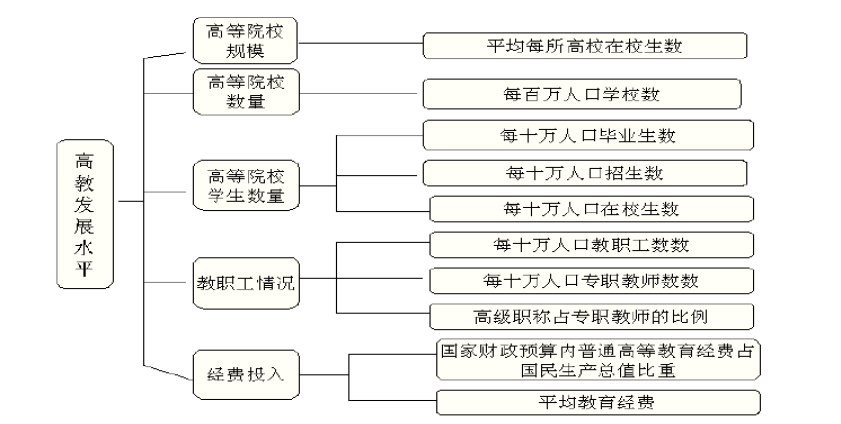
\includegraphics[scale=0.5]{Models/evaluation/PCA/Evaluation index.png}
    \caption{The ten evaluation index of higher education.}
    \label{fig:Evaluation index}
\end{figure}

(b)Data resources

Data source (see in Table \ref{tbl:Data of PCA}).

Define the ten indexes.

%%数据表格
\begin{table}[H]
    \renewcommand\arraystretch{2}   %%控制行间距
    \centering
    \begin{tabular}{|l|l|l|l|l|l|l|l|l|l|l|}    %%三列均左对齐
        \toprule  %%表格横线加粗
        \specialrule{0em}{2pt}{2pt}    %%添加透明线控制行高
        Area & $x_1$ & $x_2$ & $x_3$ & $x_4$ & $x_5$ & $x_6$ & $x_7$ & $x_8$ & $x_9$ & $x_{10}$ \\
        \specialrule{0em}{2pt}{2pt}    %%添加透明线控制行高
        \hline
        \specialrule{0em}{1pt}{1pt}    %%添加透明线控制行高
        Beijing & 5.96 & 310 & 461 & 1557 & 931 & 319 & 44.36 & 2615 & 2.20 & 13631 \\
        \hline
        Shanghai & 3.39 & 234 & 308 & 1035 & 498 & 161 & 35.02 & 3052 & 0.90 & 12665 \\
        \hline
        Tianjin & 2.35 & 157 & 229 & 713 & 295 & 109 & 38.40 & 3031 & 0.86 & 9385 \\
        \hline
        Shanxi & 1.35 & 81 & 111 & 364 & 150 & 58 & 30.45 & 2699 & 1.12 & 7881 \\
        \specialrule{0em}{1pt}{1pt}    %%添加透明线控制行高
        \bottomrule
    \end{tabular}
    \caption{Data of xxx.}
    \label{tbl:Data of PCA}
\end{table}

(c)Correlation analysis

From the data set, we can get the matrix of correlation coefficient (see in Table \ref{tbl:Matrix of PCA}).

\begin{table}[H]
    \renewcommand\arraystretch{2}   %%控制行间距
    \centering
    %% *{10}{r@{.}l|}重复10遍相同格式
    \begin{tabular}{|c|*{10}{r|}}    %%三列均左对齐
        \toprule  %%表格横线加粗
        \specialrule{0em}{2pt}{2pt}    %%添加透明线控制行高
         & $x_1$ & $x_2$ & $x_3$ & $x_4$ & $x_5$ & $x_6$ & $x_7$ & $x_8$ & $x_9$ & $x_{10}$ \\
        \specialrule{0em}{2pt}{2pt}    %%添加透明线控制行高
        \hline
        \specialrule{0em}{1pt}{1pt}    %%添加透明线控制行高
        $x_1$ & 1.000 & 0.963 & 0.984 & 0.987 & 0.999 & 1.000 & 0.892 & -0.378 & 0.801 & 0.906 \\
        \hline
        $x_2$ & 0.963 & 1.000 & 0.992 & 0.993 & 0.967 & 0.954 & 0.844 & -0.132 & 0.616 & 0.980 \\
        \hline
        $x_3$ & 0.984 & 0.992 & 1.000 & 0.999 & 0.984 & 0.978 & 0.896 & -0.208 & 0.682 & 0.949 \\
        \hline
        $x_4$ & 0.987 & 0.993 & 0.999 & 1.000 & 0.989 & 0.982 & 0.877 & -0.234 & 0.698 & 0.956 \\
        \hline
        $x_5$ & 0.999 & 0.967 & 0.984 & 0.989 & 1.000 & 0.998 & 0.869 & -0.376 & 0.795 & 0.920 \\
        \hline
        $x_6$ & 1.000 & 0.954 & 0.978 & 0.982 & 0.998 & 1.000 & 0.889 & -0.407 & 0.819 & 0.895 \\
        \hline
        $x_7$ & 0.892 & 0.844 & 0.896 & 0.887 & 0.869 & 0.889 & 1.000 & -0.225 & 0.668 & 0.720 \\
        \hline
        $x_8$ & -0.378 & -0.132 & -0.208 & -0.234 & -0.376 & -0.407 & -0.225 & 1.000 & -0.855 & -0.057 \\
        \hline
        $x_9$ & 0.801 & 0.616 & 0.682 & 0.698 & 0.795 & 0.819 & 0.668 & -0.855 & 1.000 & 0.524 \\
        \hline
        $x_{10}$ & 0.906 & 0.980 & 0.949 & 0.956 & 0.920 & 0.895 & 0.720 & -0.057 & 0.524 & 1.000 \\
        \specialrule{0em}{1pt}{1pt}    %%添加透明线控制行高
        \bottomrule
    \end{tabular}
    \caption{Matrix of correlation coefficient.}
    \label{tbl:Matrix of PCA}
\end{table}

\begin{figure}[H]
    \centering
    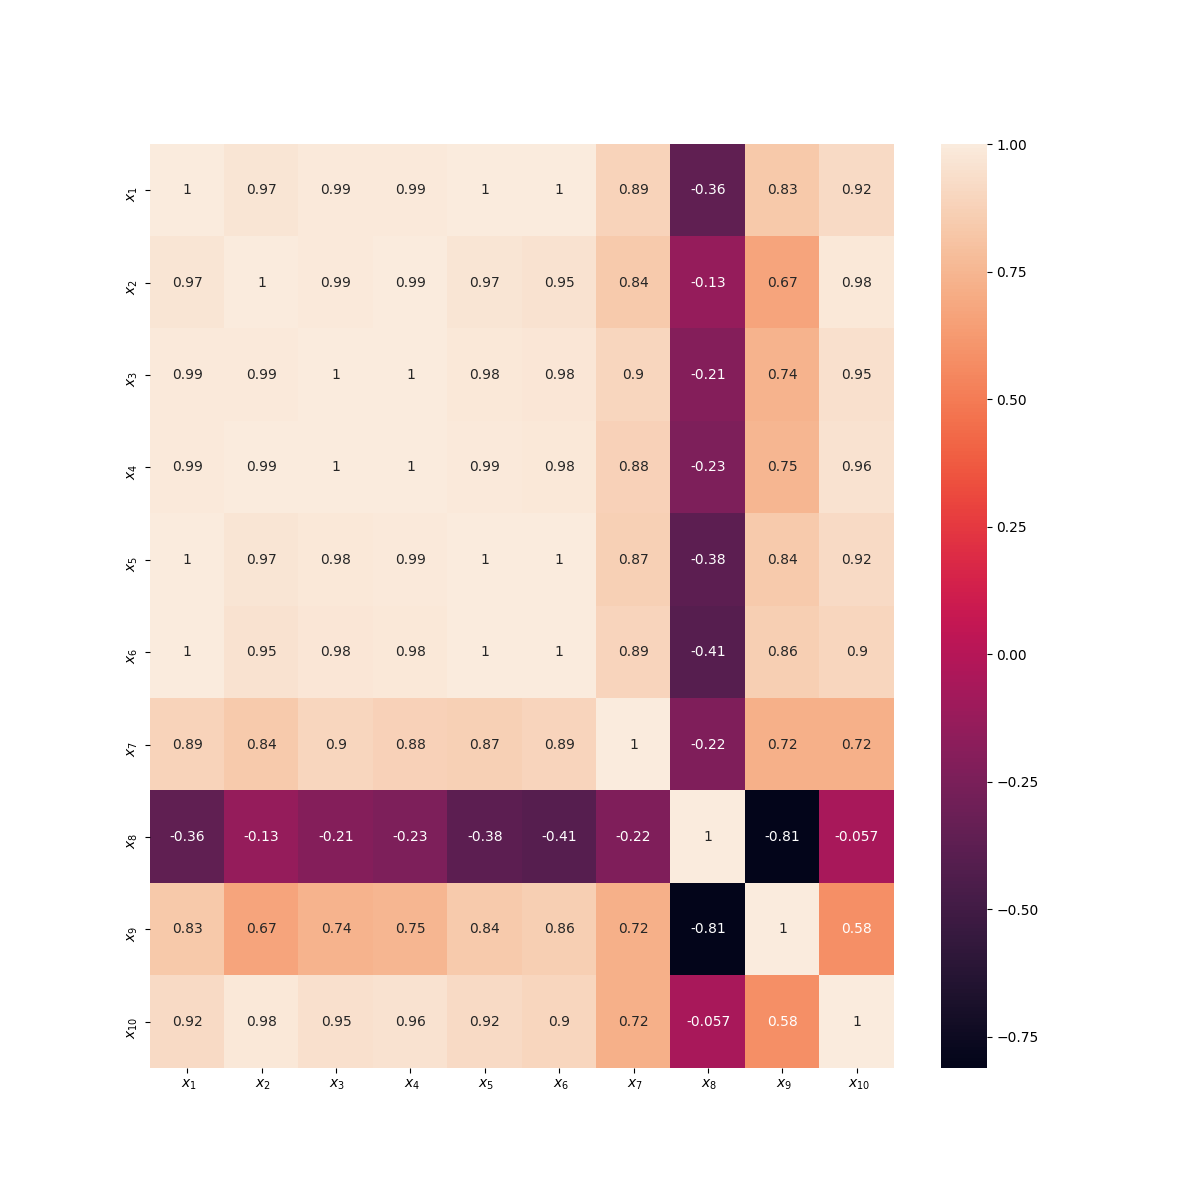
\includegraphics[width=5.5in]{Models/evaluation/PCA/PCA_correlation_analysis.png}
    \caption{PCA correlation analysis}
    \label{fig:PCA_correlation_analysis}
\end{figure}

We can see from the matrix that there exists strong correlation between some indexes. If we evaluate the problem directly, information overlap will occur, which affects the objectivity of the consequence.

(d)Conclusion

Then we use PCA to calculate eigenvalue and contribution rate (see in Table \ref{tbl:PCA consequence}).Also we can get the scree plot (see in Figure \ref{fig:Scree plot}).

\begin{table}[H]
    \renewcommand\arraystretch{2}   %%控制行间距
    \centering
    \begin{tabular}{|*{5}{r|}}    %%三列均左对齐
        \toprule  %%表格横线加粗
        \specialrule{0em}{2pt}{2pt}    %%添加透明线控制行高
        number & eigenvalue & contribution rate & cumulative contribution rate \\
        \specialrule{0em}{2pt}{2pt}    %%添加透明线控制行高
        \hline
        \specialrule{0em}{1pt}{1pt}    %%添加透明线控制行高
        1 & 8.269 & 82.690 & 82.690 \\
        \hline
        2 & 1.448 & 14.485 & 97.174 \\
        \hline
        3 & 0.283 & 2.826 & 100.000 \\
        \specialrule{0em}{1pt}{1pt}    %%添加透明线控制行高
        \bottomrule
    \end{tabular}
    \caption{PCA consequence.}
    \label{tbl:PCA consequence}
\end{table}

\begin{figure}[H]
    \centering
    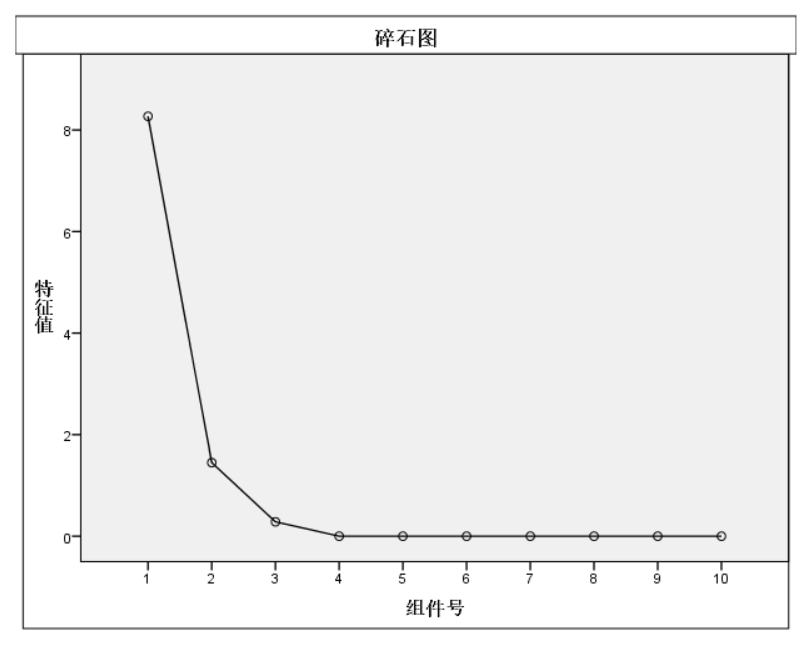
\includegraphics[scale=0.3]{Models/evaluation/PCA/Scree plot.png}
    \caption{Scree plot.}
    \label{fig:Scree plot}
\end{figure}

Through PCA, we can extract two principle components (see in Table \ref{tbl:Matrix of PCA components}).

\begin{table}[H]
    \renewcommand\arraystretch{2}   %%控制行间距
    \centering
    \begin{tabular}{|*{11}{r|}}    %%三列均左对齐
        \toprule  %%表格横线加粗
        \specialrule{0em}{2pt}{2pt}    %%添加透明线控制行高
        Component & $x_1$ & $x_2$ & $x_3$ & $x_4$ & $x_5$ & $x_6$ & $x_7$ & $x_8$ & $x_9$ & $x_{10}$ \\
        \specialrule{0em}{2pt}{2pt}    %%添加透明线控制行高
        \hline
        \specialrule{0em}{1pt}{1pt}    %%添加透明线控制行高
        1 & 1.000 & 0.966 & 0.987 & 0.990 & 0.999 & 0.999 & 0.892 & -0.365 & 0.792 & 0.912 \\
        \hline
        2 & -0.014 & 0.245 & 0.163 & 0.140 & -0.008 & -0.046 & 0.069 & 0.927 & -0.610 & 0.321 \\
        \specialrule{0em}{1pt}{1pt}    %%添加透明线控制行高
        \bottomrule
    \end{tabular}
    \caption{Matrix of components.}
    \label{tbl:Matrix of PCA components}
\end{table}

(e)Set the comprehensive evaluation system

From the coefficient of principle components, we can notice that xxx. (each component reflects which indexes)

Now, we take the contribution rare of the principle components as their ratio and get the comprehensive evaluation system.

\begin{equation*}
    Z = 0.8269y_1 + 0.1449y_2
\end{equation*}

And we get the score of the four areas (see in Table \ref{tbl:PCA score}).

\begin{table}[H]
    \renewcommand\arraystretch{2}   %%控制行间距
    \centering
    \begin{tabular}{|*{11}{r|}}    %%三列均左对齐
        \toprule  %%表格横线加粗
        \specialrule{0em}{2pt}{2pt}    %%添加透明线控制行高
        Area & Score \\
        \specialrule{0em}{2pt}{2pt}    %%添加透明线控制行高
        \hline
        \specialrule{0em}{1pt}{1pt}    %%添加透明线控制行高
        Beijing & 1.04 \\
        \hline
        Shanghai & 0.19 \\
        \hline
        Tianjin & -0.28 \\
        \hline
        Shanxi & -0.95 \\
        \specialrule{0em}{1pt}{1pt}    %%添加透明线控制行高
        \bottomrule
    \end{tabular}
    \caption{The score of the four areas.}
    \label{tbl:PCA score}
\end{table}